\section{Evaluation}
\subsection{Experimental Setup}
\textbf{Testbed.}
\system is evaluated on three different platforms.
For single-request inference, we evaluate small models on a platform equipped with an AMD EPYC 7H12 64-Core Processor and an NVIDIA RTX 3090 GPU, and evaluate large models on the Intel Xeon Gold 6330 112-core CPU paired with two NVIDIA A100 GPUs. 
For the serving scenario, we experiment on a server configured with an Intel Xeon Platinum 8358 128-core CPU and two NVIDIA A800 GPUs.

\noindent
\textbf{Search Agent Tasks.}
We build our evaluation framework on top of the ReAct agent architecture~\cite{react} (same as concurrent work~\cite{speculativeactions}) and the vLLM inference engine~\cite{vllm}, using the Wikipedia~\cite{wikipedia} API (around 1.5s per request) as the external web-search tool. 
ReAct represents the standardized reason-action workflow in modern search agents, including both workflow-level designs and reinforcement learning–based agents, making it a representative and widely adopted setting for evaluating multi-step reasoning systems. 

To comprehensively assess the performance and generality of \system, we experiment with four different LLMs: Qwen2.5-7B-Instruct (Q7), Qwen2.5-32B-Instruct (Q32)~\cite{qwen2.5}, Gemma-3-4B-it (G4), Gemma-3-27B-it (G27)~\cite{Gemma3}, we set $\text{temperature}=0$ for inference calls in main agent path to ensure result's stability.
We evaluate the agent across three search-oriented benchmarks (HotPotQA~\cite{hotpotqa}, 2WikiMultihopQA~\cite{2wikimultihop}, TriviaQA~\cite{triviaqa}), covering diverse levels of reasoning complexity and interaction depth.
For each benchmark we randomly sample a subset to construct the evaluation suite.

\noindent
\textbf{Baselines.}
We compare \system with representative baselines:
\begin{itemize}[leftmargin=*]
    \item \textbf{Naive ReAct Search Agent + vLLM~\cite{react,vllm}.} This baseline represents the standard ReAct-style search agent using vLLM as the inference engine, without any form of action speculation or system-level scheduling optimization.

    \item \textbf{Speculative Actions~\cite{speculativeactions}.} This baseline introduces speculative action execution using a predict–verify paradigm.  
    Its mechanism is equivalent to the Verified Speculation Phase in our framework. 
    This comparison isolates the benefit of our adaptive speculation strategy and system-level scheduling from previously proposed verified-only speculative action methods.
\end{itemize}
In Speculative Actions and \system, we set the sample number of speculative actions $k=3$ if not specified.

\begin{figure}
    \centering
    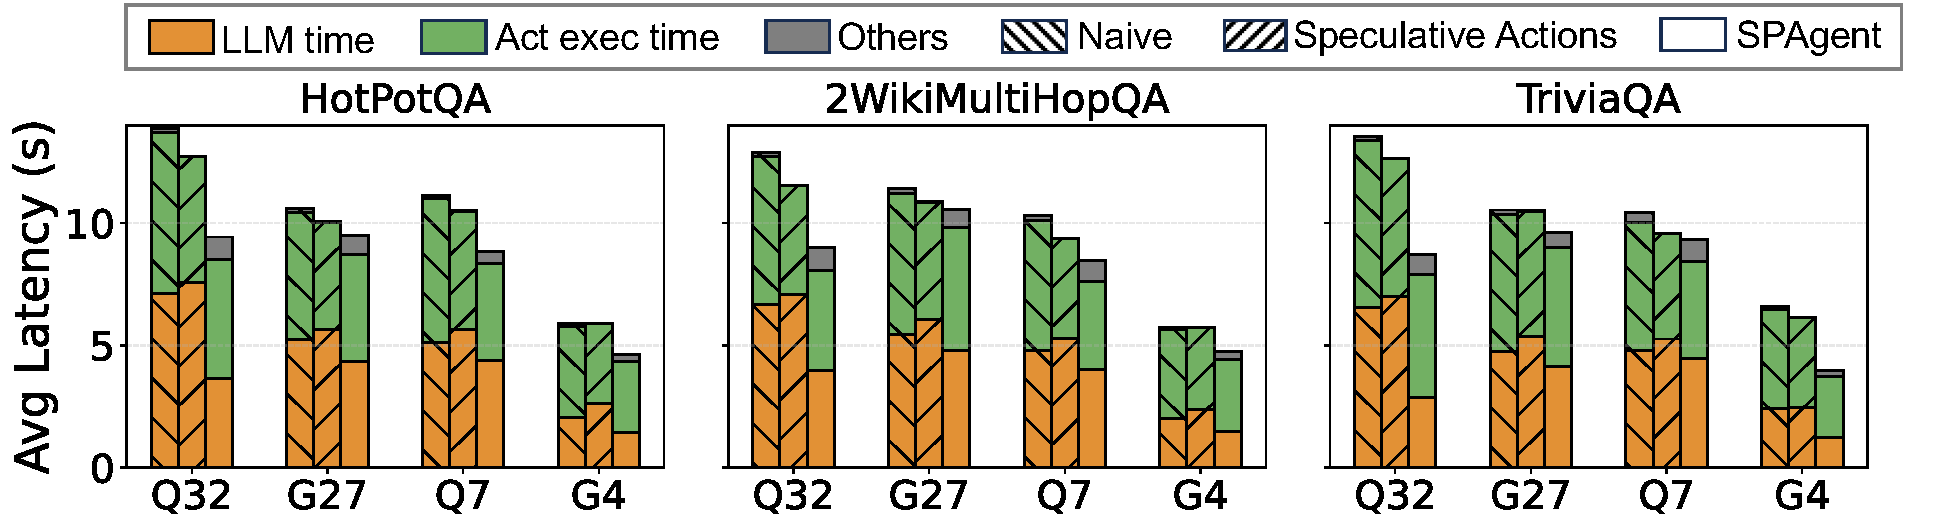
\includegraphics[width=0.99\linewidth]{figures/experiments/latency_by_dataset_grid_sp.pdf}
    % \vspace{-10pt}
    \caption{Single-request latency and component breakdown.}
    \label{fig:single}
    % \vspace{-20pt}
\end{figure}
\subsection{End-to-End Latency}
\noindent
\textbf{Single Request Inference and Latency Breakdown.}
We compare \system with Naive search agent and Speculative Action across four models and three benchmarks on RTX 3090 (Qwen2.5-7B and Gemma-3-4B) and two A100 GPUs (Qwen2.5-32B and Gemma-3-27B, tensor parallel size $TP=2$).
As shown in \Figref{fig:single}, across all settings, \system achieves $1.08\times$ to $1.65\times$ speed up conpared to the baselines.
In \Figref{fig:single}, LLM time represents for reasoning and action speculation with LLM inference; Act exec time represents the action execution time that is not overlapped with inference; Others in \system is mainly composed of model calls to get action scores.
The improvement arises from reducing both major latency components: the Aggressive Speculation Phase shortens LLM inference by skipping unnecessary reasoning in early simple steps, while the Verified Speculation Phase overlaps action execution with ongoing reasoning.
Overall, \system reduces 23.8\% LLM inference time and 29.4\% un-overlapped action execution time on average, compared with naive agent.
Speculative Actions provides only the latter benefit and increases inference latency by up to 26\% due to extra inference calls, limiting its overall effectiveness.
We also notice that models shows different preference in phase transition.
Qwen models are more likely to speculate aggressively and thus achieves larger inference-time reductions, whereas Gemma models evaluate more conservatively and revert to reasoning sooner, yielding smaller but still consistent gains.
% Breakdown analysis confirms this pattern: \system reduces both inference and action-execution time (not overlapped with inference) with minimal overhead, whereas Speculative Action reduces only the latter and increases the former, explaining its inferior end-to-end latency.

\begin{figure}[t]
    \centering
    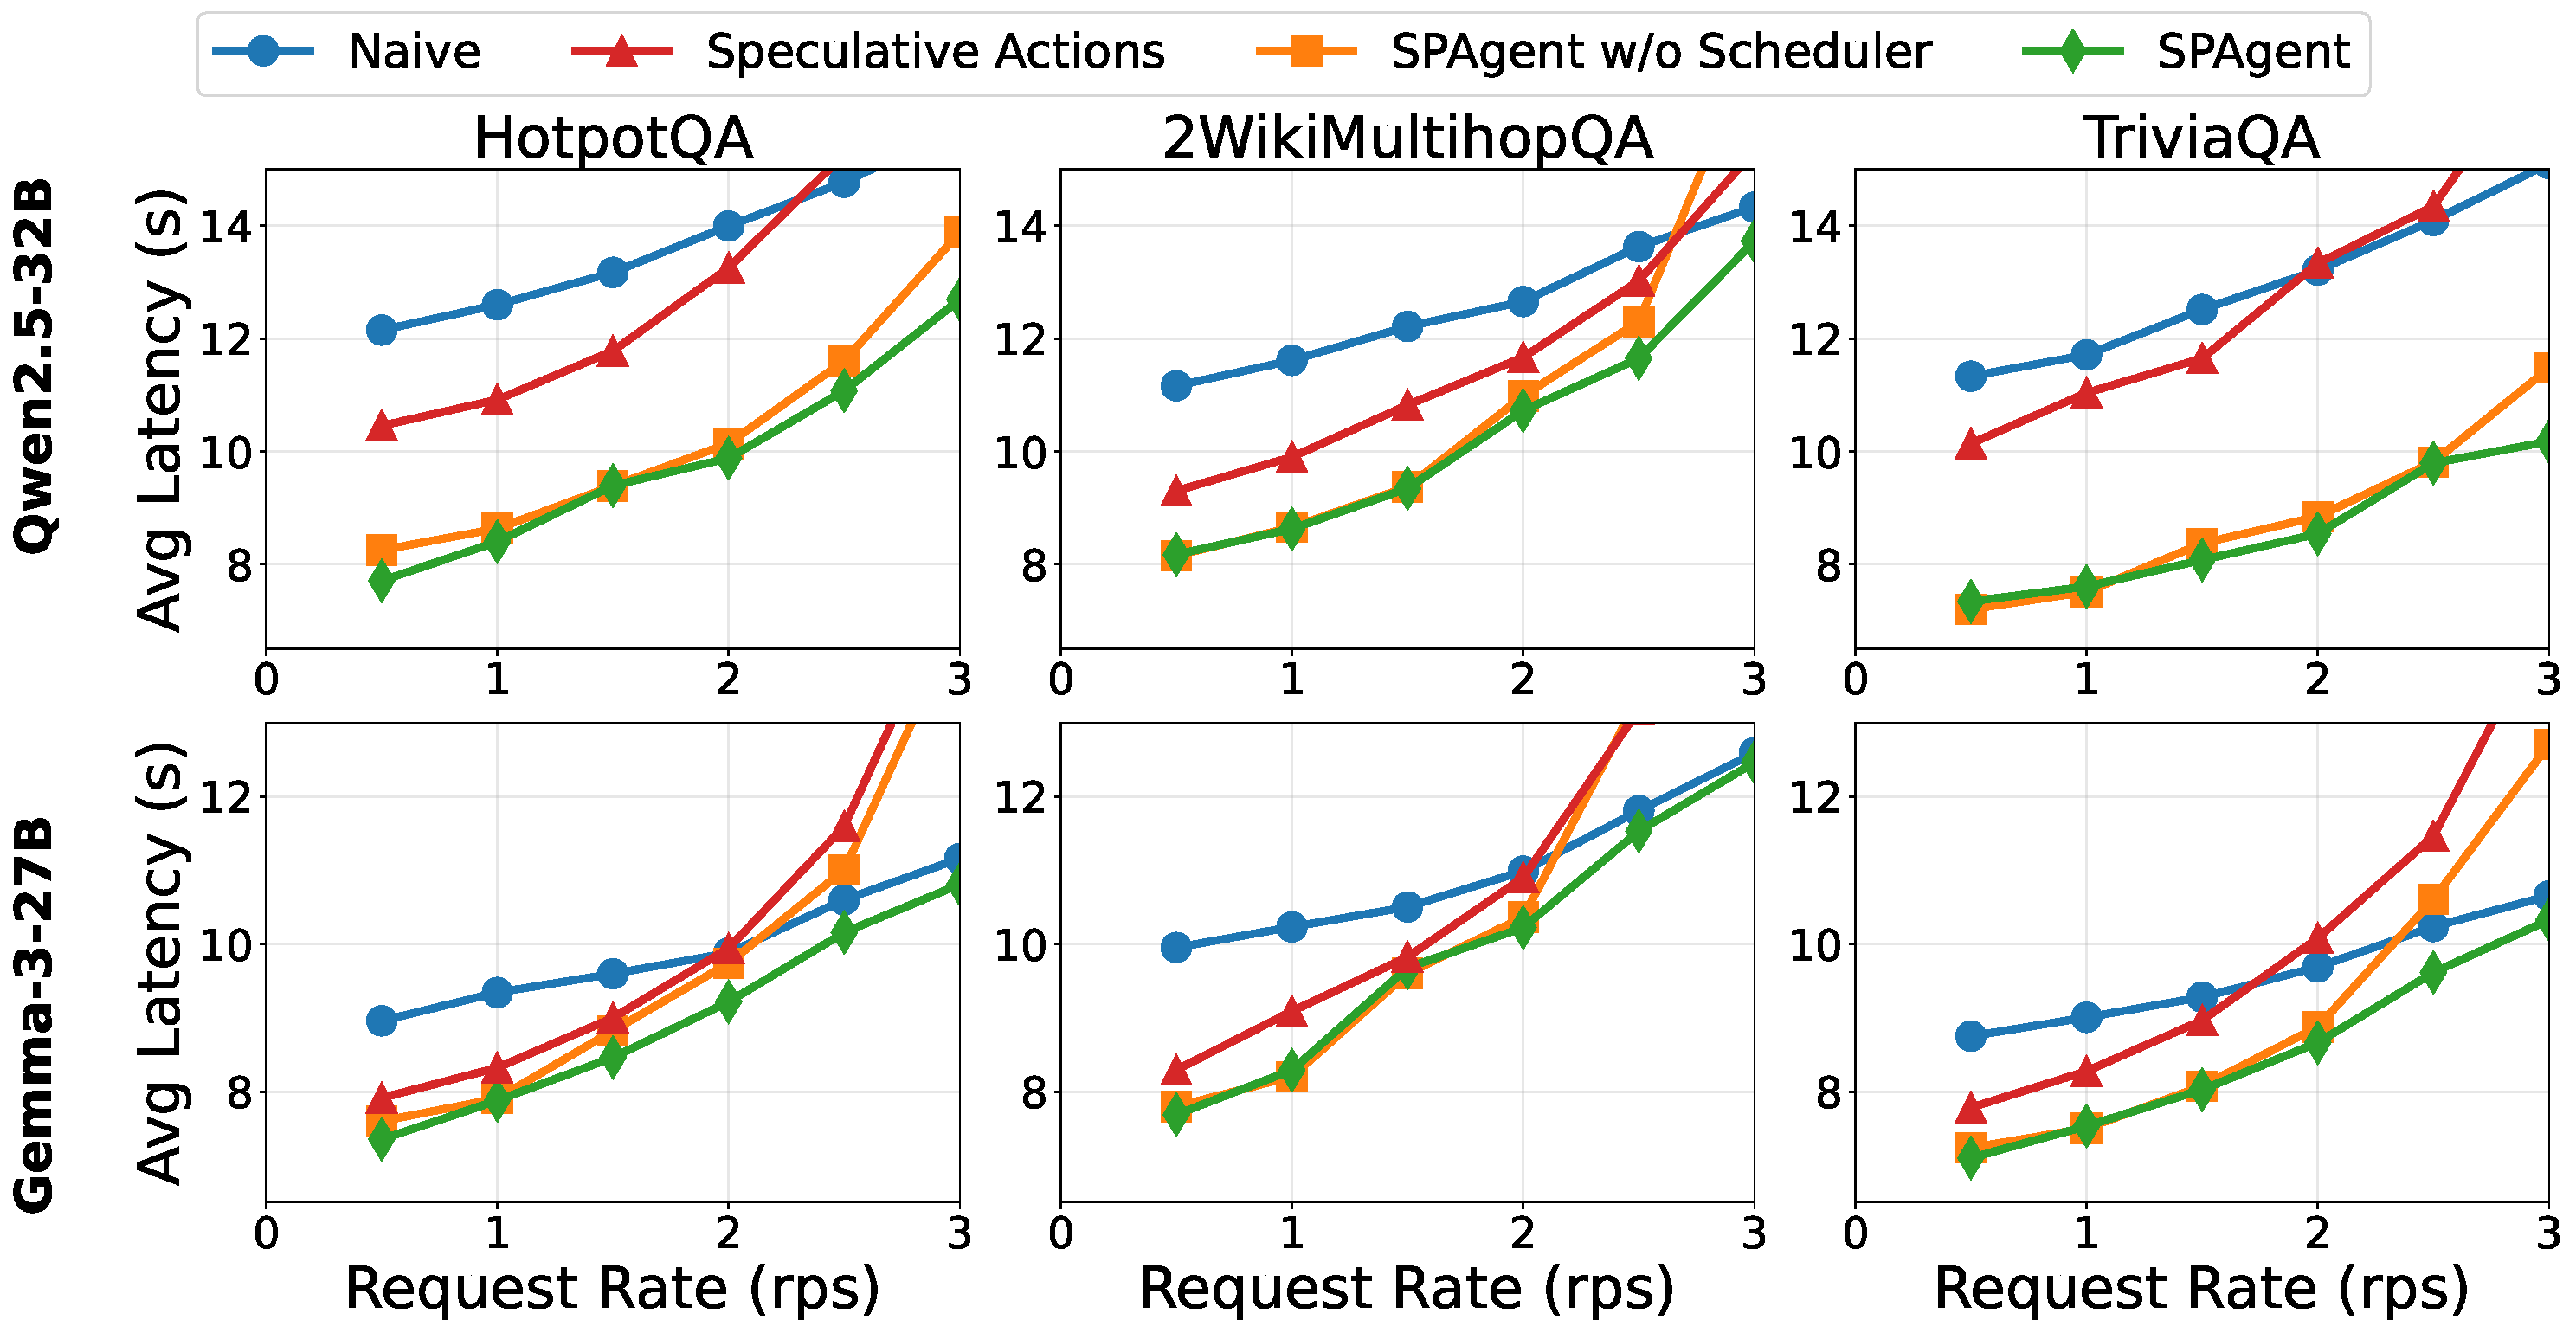
\includegraphics[width=0.99\linewidth]{figures/experiments/combined_serve_arxiv.pdf}
    % \vspace{-12pt}
    \caption{Average latency under different request rates.}
    \label{fig:serve}
    % \vspace{-12pt}
\end{figure}

\begin{table}[t]
    \centering
    \caption{Accuracy on different models and benchmarks}
    % \vspace{-10pt}
    \setlength\tabcolsep{2pt} % default value: 6pt
    \footnotesize
    \resizebox{\linewidth}{!}
    {
    \begin{tabular}{ll|ccc|cc}
        \toprule
        \multicolumn{2}{c|}{Settings}  & HotPotQA & 2WikiQA & TriviaQA & Avg. Acc. & Avg. Speedup\\
        \midrule
        \multirow{2}{*}{Gemma3-4B} & Naive & 26.2 & 25.0 & 38.4 & 29.8 & \multirow{2}{*}{$1.38\times$}\\
        & \system & 25.6 & 24.4 & 41.8 & 30.6\\
        % \hline 
        \midrule
        \multirow{2}{*}{Qwen2.5-7B} & Naive & 29.8 & 30.4 & 41.2 & 33.8 & \multirow{2}{*}{$1.19\times$}\\
        & \system & 31.0 & 30.4 & 42.0 & 34.5 \\
        % \hline
        \midrule
        \multirow{2}{*}{Gemma3-27B} & Naive & 45.2 & 46.1 & 62.6 & 51.3 & \multirow{2}{*}{$1.10\times$}\\
        & \system & 44.0 & 46.6 & 63.3 & 51.3 \\
        % \hline
        \midrule
        \multirow{2}{*}{Qwen2.5-32B} & Naive & 41.3 & 41.1 & 63.1 & 48.5 & \multirow{2}{*}{$1.48\times$}\\
        & \system & 42.8 & 42.9 & 68.1 & 51.3\\
        \bottomrule
    \end{tabular}
    }
    \label{tab:accuracy}
    % \vspace{-10pt}
\end{table}

\begin{figure*}[t]
    \begin{subfigure}[c]{0.22\linewidth}
        \centering
        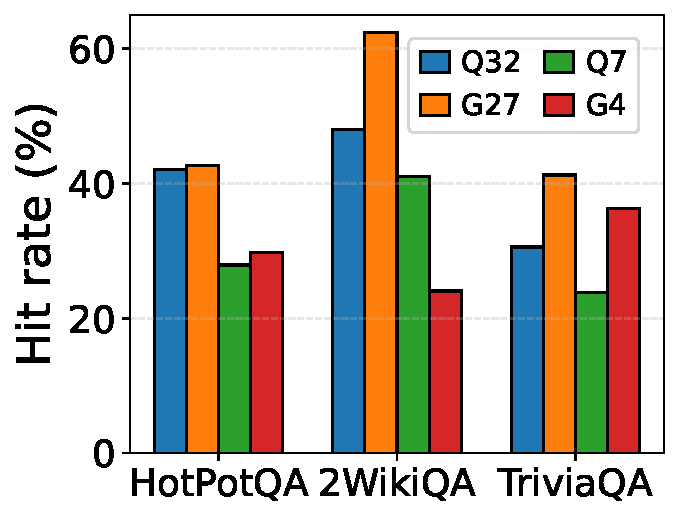
\includegraphics[width=\linewidth]{figures/experiments/hit_rate_by_dataset.pdf}
    \end{subfigure}
    \hfill
    \begin{subfigure}[c]{0.25\linewidth}
        \centering
        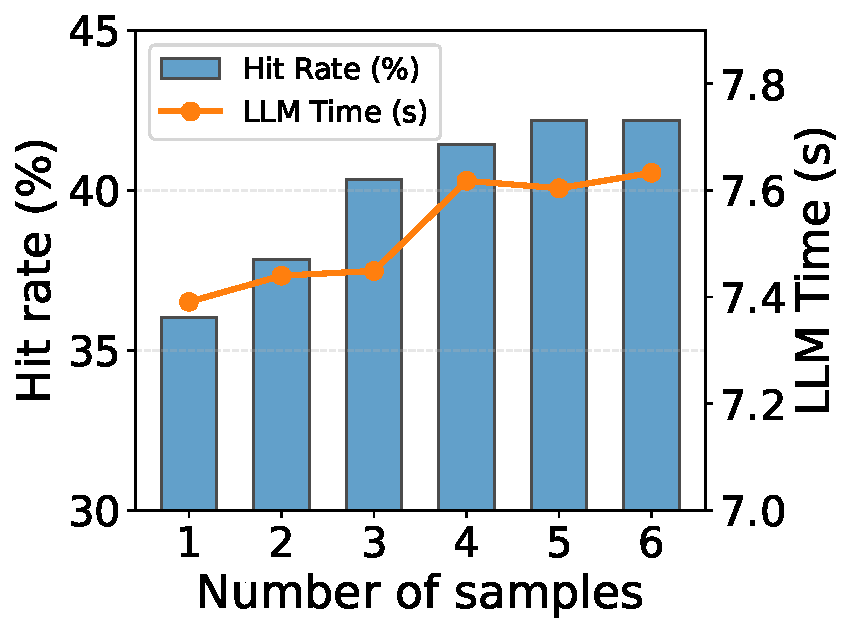
\includegraphics[width=\linewidth]{figures/experiments/llmtime_hit_rate_by_dataset.pdf}
    \end{subfigure}
    \hfill
    \begin{subfigure}[c]{0.2\linewidth}
        \centering
        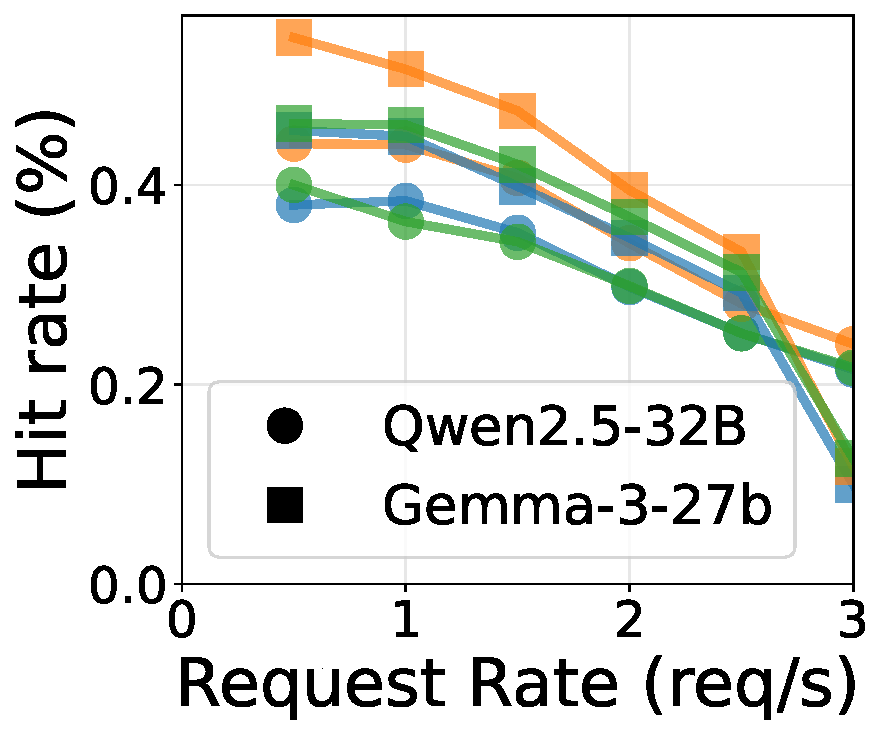
\includegraphics[width=\linewidth]{figures/experiments/hitrate_rps.pdf}
    \end{subfigure}
    % \vspace{-10pt}
    \caption{Action Buffer hit rate in different scenarios. (a) Single-request; (b) Different $k$; (c) Serving scenario.}
    \label{fig:hit_rate_eval}
    \vspace{-10pt}
\end{figure*}

\noindent
\textbf{Online Serving and System Ablation.}
We evaluate \system under online serving scenarios using and Qwen2.5-32B and Gemma-3-27B across three benchmarks on 2 NVIDIA A800 with $TP=2$, comparing against Naive search agent, Speculative Action, and an ablation without scheduling.
We generate search agent tasks' arrivals using a Poisson process, following established methodologies~\cite{vllm,fastserve}.

\Figref{fig:serve} show that \system (with or without scheduler) consistently achieves the lowest mean latency across request rates, speeding up 24.2\% on average, up to 69.6\%, compared to the naive ReAct and Speculative Actions.
Speculative Actions reduce latency compared to Naive only at low concurrency, but becomes up to 49.3\% slower than Naive once load exceeds 2 rps, as its additional inference requests slow down inference steps and overwhelm the small overlap it creates.
The no-scheduler variant suffers from the same issue: speculation increases inference load without any mechanism to regulate it, leading to significant slowdowns under high concurrency.

In contrast, \system remains robust across all loads.
At low request rates, it performs similarly to the no-scheduler variant since speculation is inexpensive. 
As concurrency rises, the scheduler selectively launches speculative requests based on engine load and expected benefit, preventing overload while still exploiting useful overlap. 
Consequently, even at 3 rps, \system avoids the latency spikes of other baselines, demonstrating that speculation is effective only when paired with load-aware scheduling.

\subsection{Accuracy Performance}

Across all evaluated models and benchmarks, \system maintains accuracy on par with the baseline, and in some cases even improves it, as shown in \Tabref{tab:accuracy}.
Notably, the Qwen2.5-32B model exhibit accuracy gains exceeding 5\% on TriviaQA, indicating that the reduced reasoning in the Aggressive Speculation Phase can occasionally enhance decision quality.
A plausible explanation is that skipping early, low-value reasoning may help the model avoid unnecessary or noisy thought chains, thereby preserving focus for later complex steps~\cite{dangeroverthinking,dontoverthinkit,adaptthink}.

The Gemma models show small declines ($\sim 1\%$) on certain benchmarks. 
The modest reductions remain within the typical variance observed when modifying agent prompts or control flows. 
Overall, the results confirm that \system does not introduce meaningful accuracy degradation while delivering substantial latency reductions.

\subsection{Action Buffer Hit Rate}

The Action Buffer hit rate is the proportion of actions generated by the main agent path in the Verified Speculation Phase that can reuse speculative actions already stored in the buffer.
\Figref{fig:hit_rate_eval}a shows Action Buffer hit rate in single-request inference. 
Across models and benchmarks, the hit rate is typically around 40\%, indicating that speculative actions often match the final actions and confirming the practical effectiveness of action-level speculation. 
Note that this metric excludes steps handled by the Aggressive Speculation Phase, which contributes substantially to speedup, so hit rate should not be interpreted as the full extent of speculation’s benefit.
We also evaluate the influence of sample number $k$, shown in \Figref{fig:hit_rate_eval}b.
As the number of sampled speculative actions $k$ increases, the hit rate improves but exhibits diminishing marginal returns, while the additional speculative inference introduces non-negligible overhead. 
Therefore, we set $k=3$ by default, which provides a favorable balance between accuracy gains and computational cost.
In the serving scenarios in \Figref{fig:hit_rate_eval}c (shapes denote models, colors for benchmarks), hit rates naturally decline as request rates increase because the scheduler intentionally suppresses speculative launches under high load to avoid harming inference latency. 
The sharper reduction observed on Gemma model reflects a more conservative scheduling response. 
Overall, these trends demonstrate both the inherent viability of speculative actions and the scheduler’s ability to adapt speculation intensity to system conditions.
